\begin{figure}[h!]
\label{fig:mac-grid}
\centering
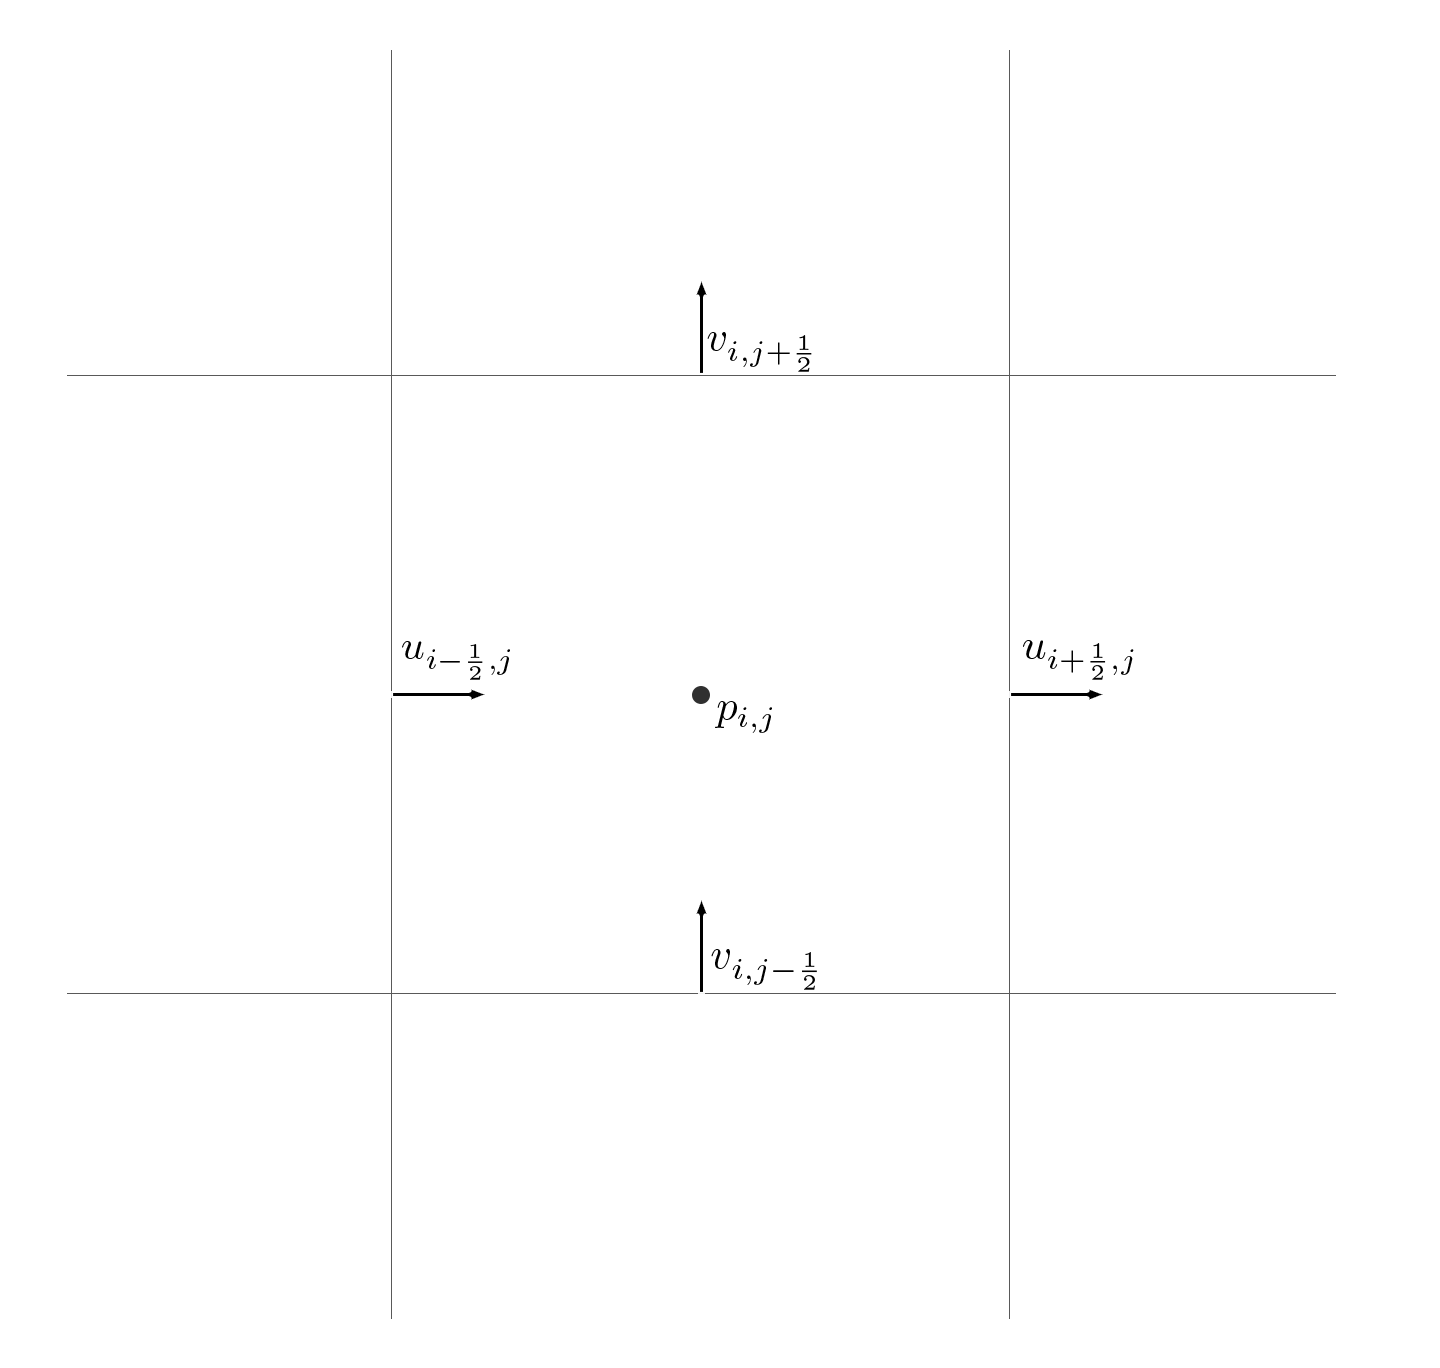
\includegraphics[width=0.6\textwidth]{mac.png}
\caption{2D MAC grid, $p$ is pressure, $u$ and $v$ are velocity components. Half indices are used for illustrative purposes, an implementation should use whole indices.}
\end{figure}

In order to discretize the navier-stokes equations spatially, a technique called MAC (Marker And Cell) is often used. Space is quantified in equally sized cells, sampled quantities such as velocity components and pressure are spread out at different locations in the grid, see fig. \ref{fig:mac-grid}. The pressure is stored in the center of each cell and the velocity is split componentwise and placed at cell faces orthogonal to its direction. 
The placement of velocity vectors and pressure might seem a bit odd but makes the central difference accurate for the pressure gradient and velocity divergence \cite{bridson}, it's easy to find out how much is flowing in or out of a cell which is essential when doing the pressure update. 

A less appealing consequence on the other hand is that a velocity vector can not be accessed directly, it requires interpolation each time since the components are separated. Additional properties might be stored in the grid depending on the type of fluid being simulated, in the case of a fire simulation where buoyancy is a distinguishing feature that can be mimicked by evaluating the local temperature difference, temperature can be stored in the cell center. To track the interface between the blue-core and hot gaseous medium the level-set method is used. The ghost fluid method described in more detail in \ref{sec:method_two_phase_flow} requires a duplicate of each velocity component to account for discontinuous density at the fuel interface.


